
MulVal produces multiple output files when it generates an attack graph. The following section documents the process used to generate the transition matrix required for input to the CSAF using the output from MulVal. Running MulVal with the \verb|-l| or \verb|-v| option will create the necessary output files.


% \begin{algorithm}
% \caption{Calculate Transition Matrix}
% \label{genTransMatrix}

% \begin{algorithmic}
% \REQUIRE ARCS.CSV and VERTICES.CSV
% \FOR{vertex in VERTICES.CSV}
%  \STATE parseVertex() \COMMENT{store NodeID, NodeType, and NodeText}
% \ENDFOR

% \FOR{arc in ARCS.CSV}
%  \STATE parseArc() \COMMENT{ store immediate predecessors and successors}
% \ENDFOR

% \STATE n = count(orNodes) \COMMENT{*only include exploitable OR nodes}
% \STATE tmatrix = zeroes(n,n) \COMMENT{initialize $n$x$n$ matrix with 0's}

% \FOR{each OR node}
%  \FOR{each parent OR node}
% %  \STATE tmatrix[parentOR][currentOR]= exploit probability \COMMENT{write incoming exploit probability to transition matrix}
%  \STATE tmatrix[parentOR][currentOR]= exploit success probability
%  \ENDFOR
%  \STATE tmatrix[currentOR][currentOR]= exploit failure probability % \COMMENT{$1 -  $ exploit probability}
% \ENDFOR
%  \RETURN TransitionMatrix.csv
%  \end{algorithmic}
% \end{algorithm}

\begin{algorithm}
\caption{Reduce Transition Matrix}
\label{genTransMatrix}

\begin{algorithmic}
\REQUIRE ARCS, VERTICES
\STATE G = DirectedGraph(VERTICES, ARCS)
% \STATE source = Attacker Location
% \STATE sink = Attacker Target
\STATE ANDs = $v \in VERTICES : v = \textit{MulVal Rule}$
\STATE ORs = $v \in VERTICES : v = \textit{MulVal State}$
\STATE LEAFs = $v \in VERTICES : v = \textit{MulVal Fact}$

\FOR{v in ANDs} 
 \STATE score(v, ScoringStrategy)
 \STATE setEgressEdgeScores(v)
\ENDFOR
\STATE G.remove(LEAFs) 
\STATE ScoredRules = $v \in ANDs : \textit{ v.score is not None}$
\WHILE{ ANDs != ScoredRules}
\FOR{v in ScoredRules, p in (v.parentANDs \\ not in ScoredRules) }
    \STATE coalesce(p.parentANDs, v)
\ENDFOR
\ENDWHILE

\FOR{v in ANDs} 
 \STATE coalesce(v.parentOR, v.childOR)
\ENDFOR
% \STATE G.remove(ANDs) 

\FOR{edge in ARCs} 
 \STATE G.setEdgeWeight(edge, weight)
\ENDFOR

 \RETURN adjacencyMatrix(G)
 \end{algorithmic}
\end{algorithm}


To demonstrate, we calculate the transition matrix for the simple attack graph example included with the MulVal package and documented in Section \ref{subsec:background:ag}. We adopt the loop removal approaches put forth in \cite{Ou_Boyer_McQueen_2006} to discard cycles in the attack graph before translating to the transition matrix. Logic reduction techniques have been identified in \cite{Hong_Kim_Takaoka_2013} to reduce the state space of the attack graph.  Our implementation follows the methodology implied in \cite{Abraham_2016} by coalescing nodes that are reachable post-exploit without requiring further compromise (so called 'multihop access' nodes) to further reduce state space. Also, while the effects of various CVSS based weighting schemes are explored in \cite{Sembiring_Ramadhan_Gondokaryono_Arman_2015}, our design uses a simple normalized average when assigning probabilities among multiple outbound vulnerabilities.

Tables \ref{tab:eg_verts} and \ref{tab:eg_arcs} give the MulVal output generated for the attack graph nodes and edges shown in Figure \ref{fig:transGraph}. The resulting unweighted transition matrix is shown in Table \ref{tab:eg_utransmatrix}. This is a square $n$x$n$ matrix which contains only OR nodes that can be reached through successful exploitation.
Referring again to Figure \ref{fig:tg_001}:
\begin{enumerate}
\item Node 0 is the attacker's origin
\item From node 0, only node 13 is reachable
\item From node 13, either node 10 or node 5 can be reached
\begin{itemize}
\item Node 10 is immediately available given the attacker's current privilege level, so no exploit is necessary. We coalesce this node in the path between node 13 and node 8 in the transition matrix.
\item Node 5 is directly reachable from node 13 and node 8
\end{itemize}
\item Node 3 is only reachable from node 5
\item Node 1 (target) is only reachable from node 3
\end{enumerate}


\begin{table}[ht]
\tiny\centering
\caption{Unweighted Transition Matrix}
\label{tab:eg_utransmatrix}
\resizebox{.4\textwidth}{!}{%
\begin{tabular}{|l|llllll}
\toprule
NodeID & 0  & 13 & 8 & 5 & 3 & 1 \\ \midrule
0 & 1 & 1 & 0  & 0  & 0 & 0 \\ 
13 & 0 & 1 & 1 & 1 & 0 & 0   \\
8 & 0 & 0 & 1 & 1 & 0 & 0 \\
5 & 0 & 0 & 0 & 1  & 1 & 0 \\
3 & 0 & 0 & 0 & 0 & 1 & 1 \\ 
1 & 0 & 0 & 0 & 0 & 0 & 1               
\end{tabular}%
}
\end{table}

\begin{table}[ht]
\tiny\centering
\caption{Weighted Transition Matrix}
\label{tab:eg_wtransmatrix}
% \flushleft
\resizebox{.4\textwidth}{!}{%
\begin{tabular}{@{}llllll@{}}
\toprule
0 & 13 & 8 & 5 & 3 & 1 \\ \midrule
0 & 1 & 0.0 & 0.0 & 0.0 & 0.0 \\
0.0 & 0.24 & 0.22 & 0.55 & 0.0 & 0.0 \\
0.0 & 0.0 & 0.29 & 0.71 & 0.0 & 0.0 \\
0.0 & 0.0 & 0.0 & 0.62 & 0.38 & 0.0 \\
0.0 & 0.0 & 0.0 & 0.0 & 0.5 & 0.5 \\
0.0 & 0.0 & 0.0 & 0.0 & 0.0 & 1.0 \\ \bottomrule            
\end{tabular}
}
% \caption{weighted transition matrix $P$}
\label{tab:wt_transmatrix}
% \end{subtable}
\label{fig:eg_tmatrix}
\end{table}


We see the unweighted transition matrix in Table \ref{tab:eg_utransmatrix} is a direct transcription of the vulnerable nodes in the attack graph and their reachability. In the next step we assign probabilities of successful exploitation for use in simulations, so the diagonal is populated with 1's here to hold the probability an attacker fails to compromise the subsequent step and remains at the current state.

Following the simple weighting strategy identified in \cite{Abraham_2016} we let the probabilities of the transition matrix $P$ be determined by $p(i,j)= \frac{e_j}{\sum_{k=1}^{n}e_k}$ where $n$ is the number of outgoing edges from a given state $i$, and $j$ is the exploitability score for a vulnerability in state $j$ determined by its CVSS value. 

In the event a CVSS score is unavailable in the NVD, we provide several mechanisms to control the weight assigned to transitions by taking advantage of the 'hypothetical vulnerability' capabilities built into MulVal. For example, 'CAN-2002-0392' uses the (now deprecated) CANdidate prefix for the 'CVE-2002-0392' vulnerability and is not found in the current NVD database sync. Often products with a large user base will maintain their own list of public vulnerabilities that don't get assigned a CVE identifier. So, to specify individual vulnerability identifiers and scores (or to override existing ones) we can load a dictionary of vulnerabilities from configuration that will be checked before looking up values in the local NVD instance. We also allow default scores for individual vulnerability classes (eg 'Trojan horse installation') and the ability to define a catchall score or 'alert and exit' mechanism if no matching vulnerability is found. For the following manually entered exploitability scores we obtain the weighted transition matrix found in Table \ref{tab:wt_transmatrix}:


\begin{itemize}
\item 'CAN-2002-0392' = 7.5
\item 'direct network access' = 10
\item 'NFS shell' = 9.5
\item 'execCode implies file access' = 7.8
\item 'NFS semantics' = 9.6
\item 'Trojan horse installation' = 5
\item 'vulID' = 1 \# fallback value for undefined vulnerabilities
\end{itemize}




% \begin{table}[H]
% \begin{tabular}{@{}llllll@{}}
% \toprule
% 15 & 13 & 8 & 5 & 3 & 1 \\ \midrule
% 0.5714285714285714 & 0.42857142857142855 & 0.0 & 0.0 & 0.0 & 0.0 \\
% 0.0 & 0.4166666666666667 & 0.05555555555555555 & 0.5277777777777778 & 0.0 & 0.0 \\
% 0.0 & 0.0 & 0.11363636363636363 & 0.8863636363636362 & 0.0 & 0.0 \\
% 0.0 & 0.0 & 0.0 & 0.473972602739726 & 0.5260273972602739 & 0.0 \\
% 0.0 & 0.0 & 0.0 & 0.0 & 0.6575342465753424 & 0.3424657534246575 \\
% 0.0 & 0.0 & 0.0 & 0.0 & 0.0 & 1.0 \\ \bottomrule            
% \end{tabular}
% \caption{weighted transition matrix $P$}
% \label{fig:eg_transmatrix}
% \end{table}

% \begin{table}[H]
% \centering
% \begin{tabular}{@{}llllll@{}}
% \toprule
% 15 & 13 & 8 & 5 & 3 & 1 \\ \midrule
% 0.571 & 0.428 & 0.0 & 0.0 & 0.0 & 0.0 \\
% 0.0 & 0.416 & 0.055 & 0.527 & 0.0 & 0.0 \\
% 0.0 & 0.0 & 0.113 & 0.886 & 0.0 & 0.0 \\
% 0.0 & 0.0 & 0.0 & 0.473 & 0.526 & 0.0 \\
% 0.0 & 0.0 & 0.0 & 0.0 & 0.657 & 0.342 \\
% 0.0 & 0.0 & 0.0 & 0.0 & 0.0 & 1.0 \\ \bottomrule            
% \end{tabular}
% \caption{weighted transition matrix $P$}
% \label{fig:eg_transmatrix}
% \end{table}

Starting at the top row, from node 15 (direct internet access) an attacker can attempt to exploit node 13 (remote code execution). The probability the attack is successful is $\frac{7.5}{7.5 + 10}=0.42857\dots$ and the probability the attack fails is $1 - \frac{7.5}{7.5 + 10} = 0.5714\dots$ Obviously care should be taken when assigning exploitability scores to hypothetical vulnerabilities to yield a sufficiently realistic view of the network security posture. We have designed the framework to be configurable both in the weights assigned to vulnerability classes and to the weighting strategy in general as described in Section \ref{subsec:contribs:deploy}. The remainder of this paper uses the weighting strategy described in the CSAF, and research into optimized strategies is ongoing. 



% \begin{figure}
% \begin{subfigure}[t]{.94\textwidth}
% 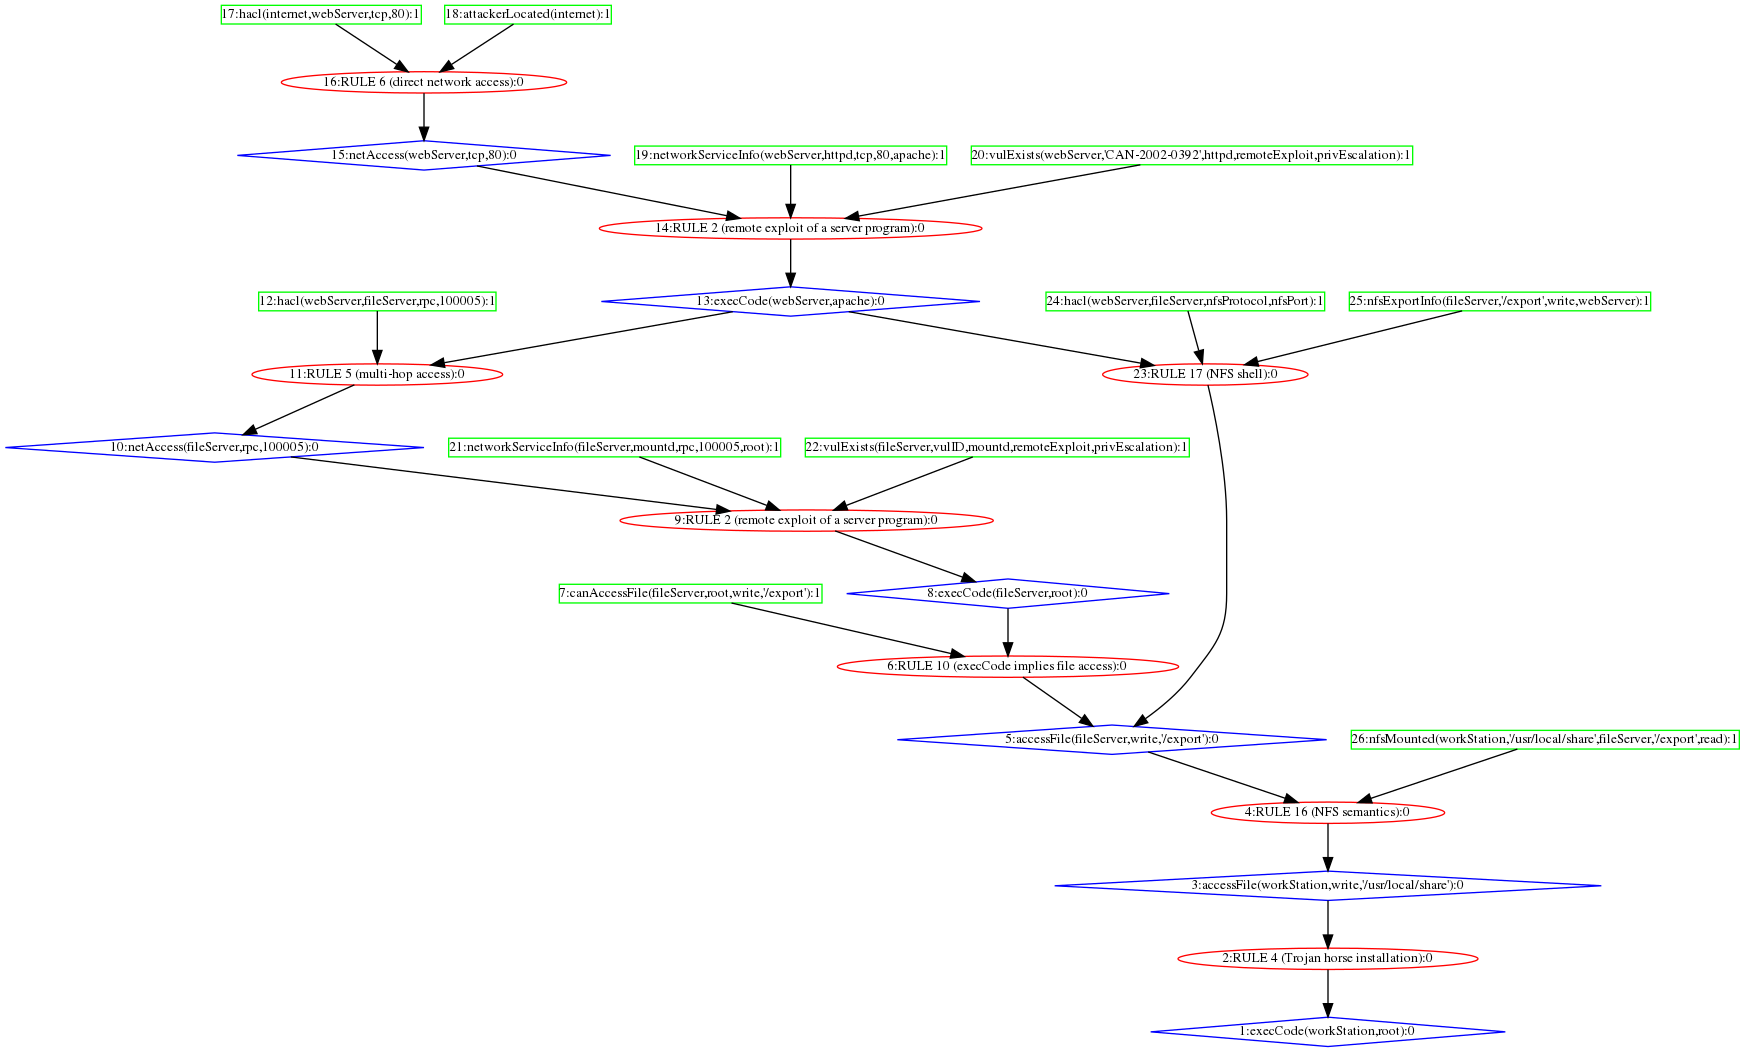
\includegraphics[width=.8\linewidth]{resource/img/ch_background/sdn_analytics/tmatrix_graphs/nameMe_001_orig.png}
% \end{subfigure}
%     \caption{Attack Graph Reduction}
%     \label{fig:transGraph}
% \end{figure}

% \begin{figure}
% 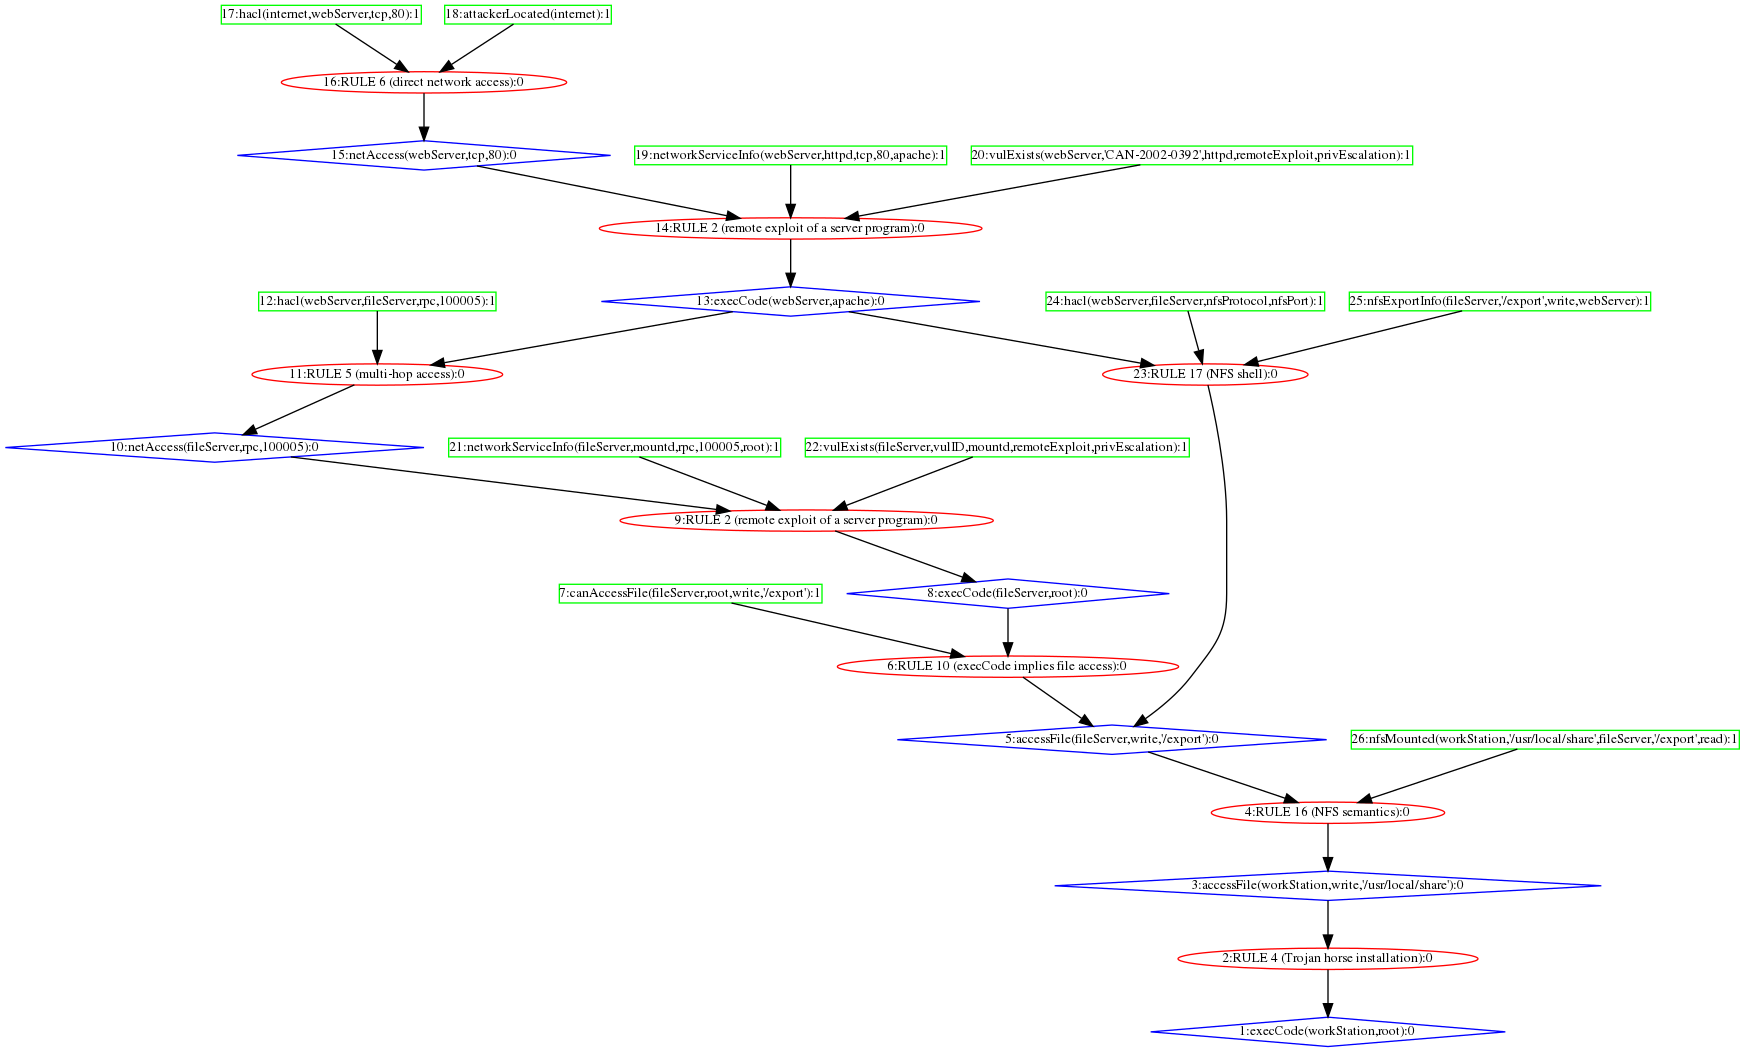
\includegraphics[width=.8\linewidth]{resource/img/ch_background/sdn_analytics/tmatrix_graphs/nameMe_001_orig.png}
    % \begin{subfigure}[t]{.94\textwidth}
    %     \centering
    %     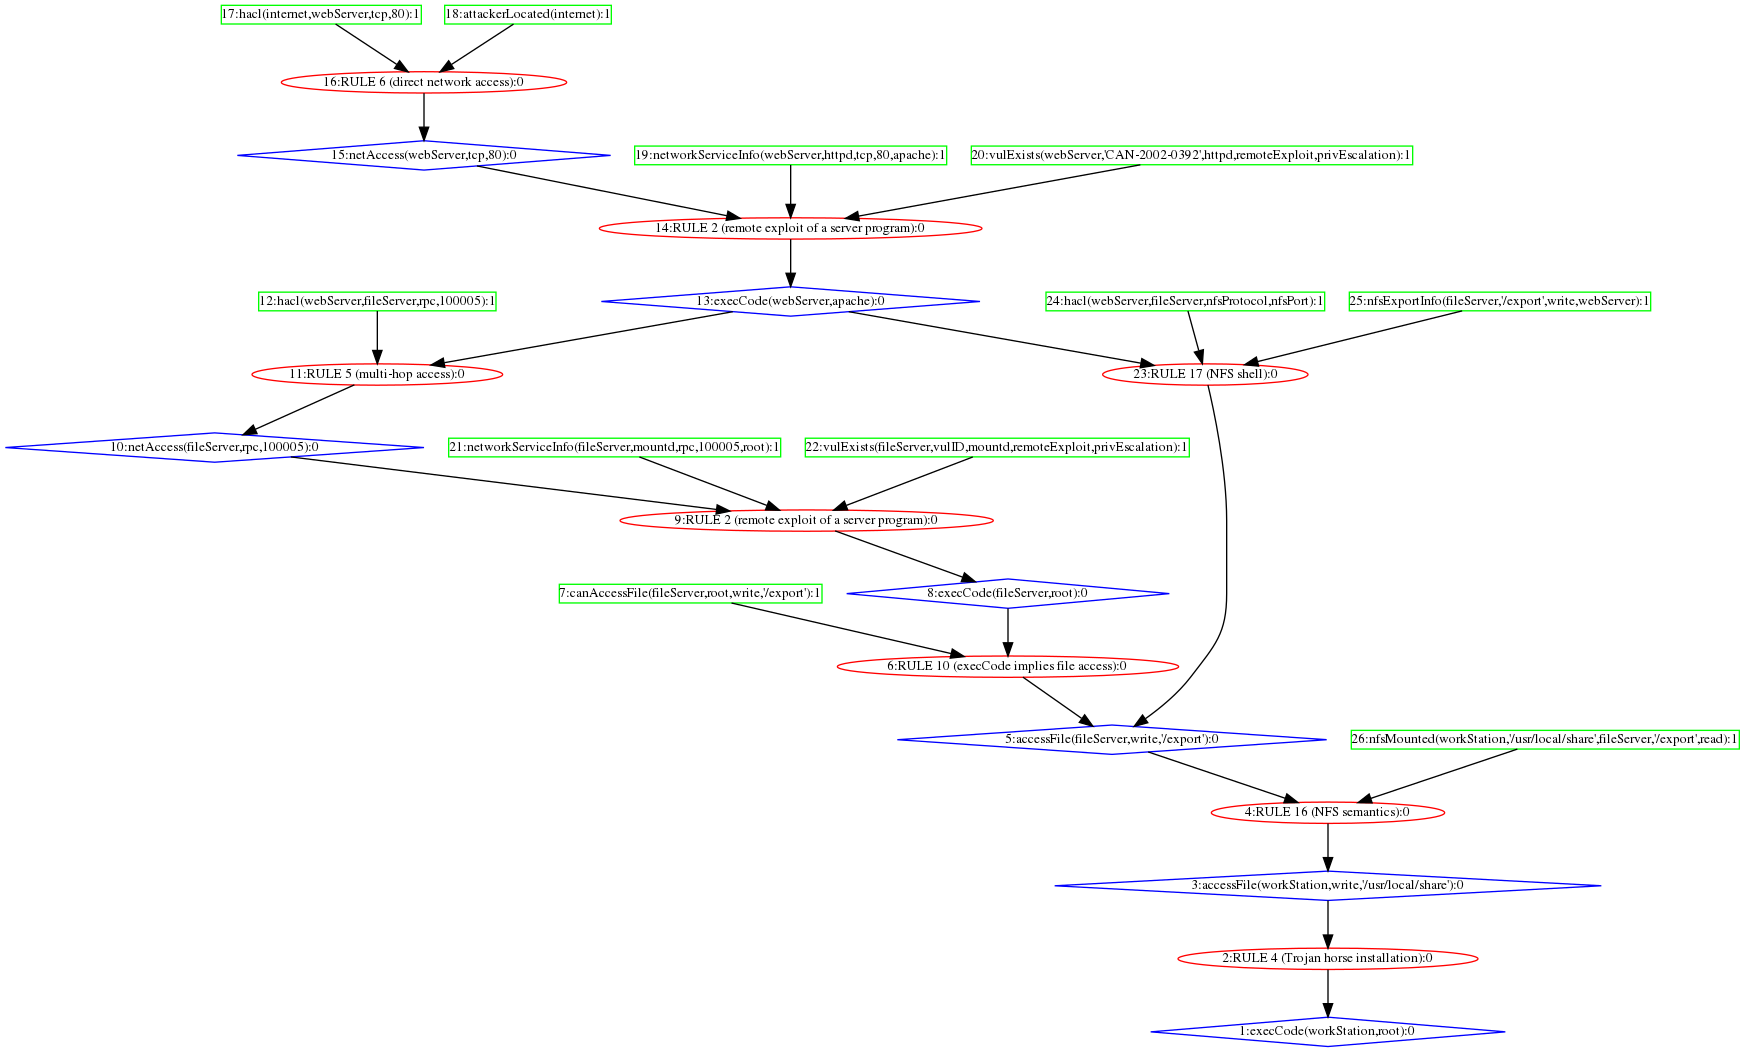
\includegraphics[width=.8\linewidth]{resource/img/ch_background/sdn_analytics/tmatrix_graphs/nameMe_001_orig.png}
    %     \caption{Attack graph produced by MulVal} 
    %     \label{fig:tg_001}
    % \hfill
    % \vspace{.2cm}
    % \end{subfigure}
    % \centering
    % \begin{subfigure}[t]{0.3\textwidth}
    %     % \centering
    %     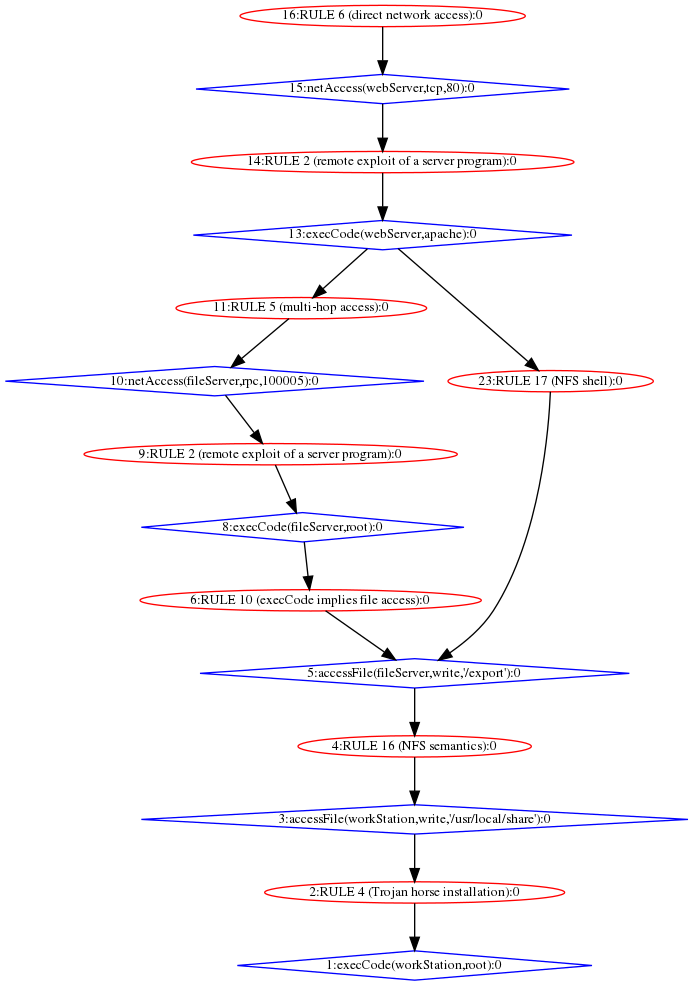
\includegraphics[width=\linewidth]{resource/img/ch_background/sdn_analytics/tmatrix_graphs/nameMe_002_pruneLEAFs.png} 
    %     %\caption{LEAFs scored \& pruned} 
    %     \label{fig:tg_002}
    % \end{subfigure}
    %       \begin{subfigure}[t]{0.3\textwidth}
    %     \centering
    %     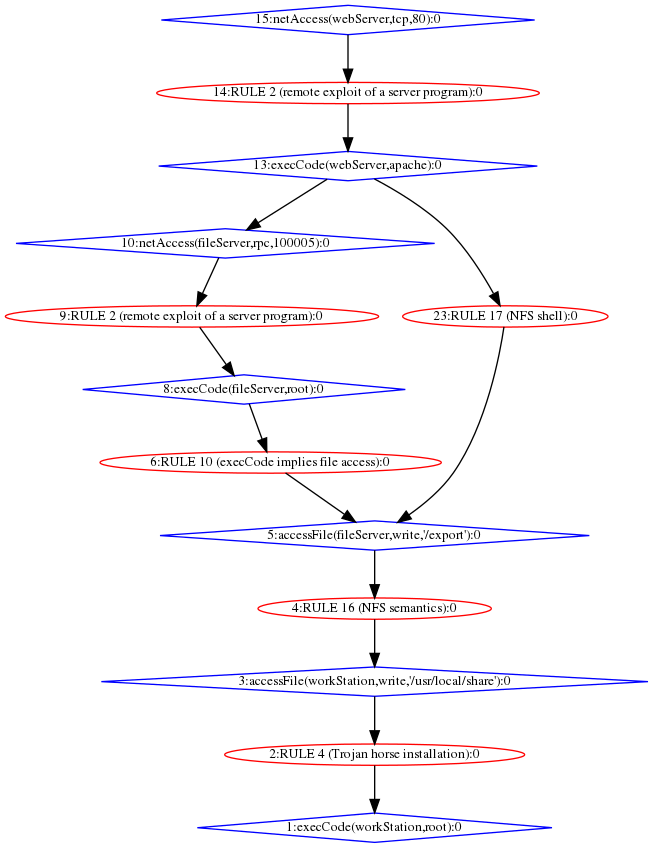
\includegraphics[width=\linewidth]{resource/img/ch_background/sdn_analytics/tmatrix_graphs/nameMe_003_coalesceANDs.png} 
    %     %\caption{Merge non-exploit ANDs}
    %     \label{fig:tg_003}
    % \end{subfigure}
    %  \begin{subfigure}[t]{0.3\textwidth}
    %     \centering
    %     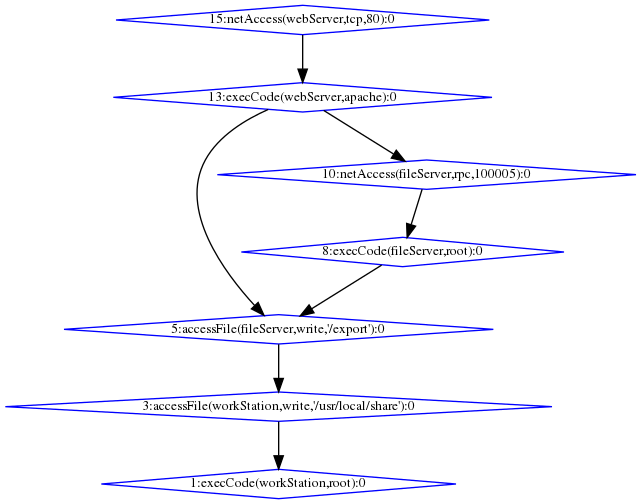
\includegraphics[width=\linewidth]{resource/img/ch_background/sdn_analytics/tmatrix_graphs/nameMe_004_scoreANDs.png} 
    %     %\caption{Merge remaining ANDs} 
    %     \label{fig:tg_004}
    % \end{subfigure}
    % \hfill
    % \vspace{.2cm}
    % \centering
    % \begin{subfigure}[t]{0.3\textwidth}
    %     \centering
    %     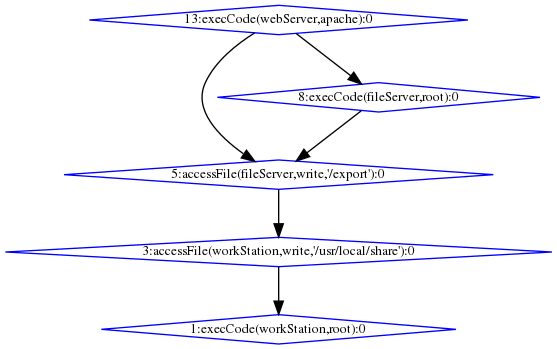
\includegraphics[width=\linewidth]{resource/img/ch_background/sdn_analytics/tmatrix_graphs/nameMe_005_coalesceORs.png} 
    %     %\caption{Merge remaining ORs} 
    %     \label{fig:tg_005}
    % \end{subfigure}
    % \begin{subfigure}[t]{0.3\textwidth}
    %     \centering
    %     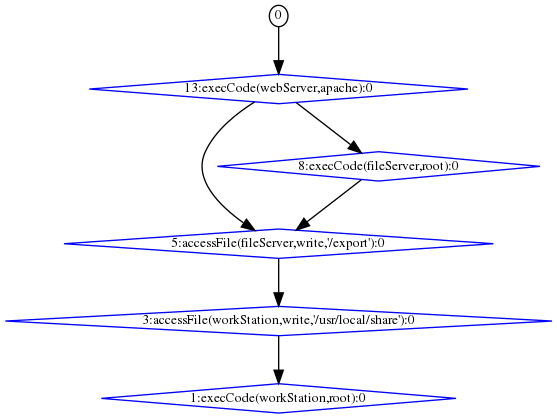
\includegraphics[width=\linewidth]{resource/img/ch_background/sdn_analytics/tmatrix_graphs/nameMe_006_addOrigin.png} 
    %     %\caption{Add pseudo-root} 
    %     \label{fig:tg_006}
    % \end{subfigure}
    %     \begin{subfigure}[t]{0.3\textwidth}
    %     \centering
    %     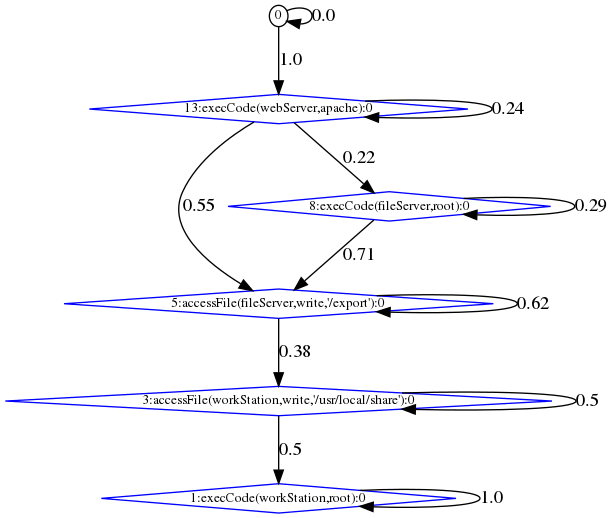
\includegraphics[width=\linewidth]{resource/img/ch_background/sdn_analytics/tmatrix_graphs/nameMe_007_weighEdges.png} 
    %     %\caption{Calculate advance probs} 
    %     \label{fig:tg_008}
    % \end{subfigure}
%     \hfill
%     \caption{Attack Graph Reduction}
%     \label{fig:transGraph}
% \end{figure}







\begin{figure}
    \begin{subfigure}[t]{.94\textwidth}
        \centering
        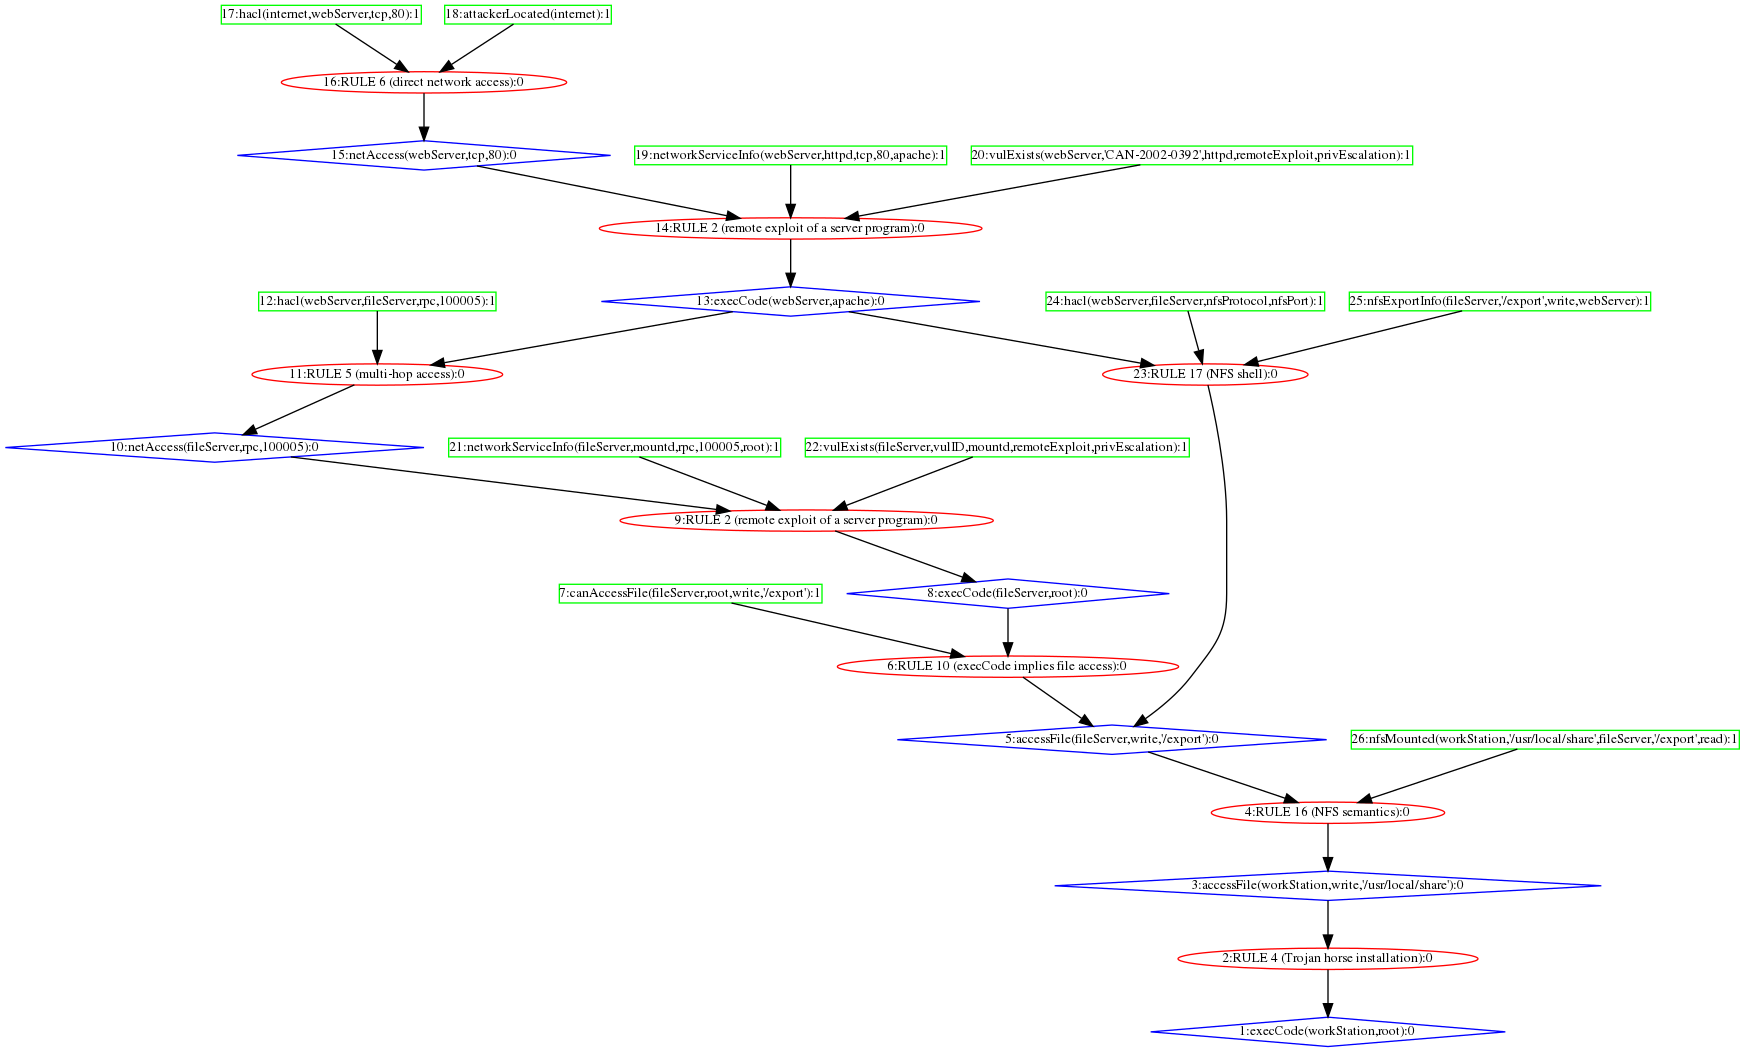
\includegraphics[width=.8\linewidth]{resource/img/ch_background/sdn_analytics/tmatrix_graphs/nameMe_001_orig.png}
        \caption{Attack graph produced by MulVal} 
        \label{fig:tg_001}
    \hfill
    \vspace{.2cm}
    \end{subfigure}
    \centering
    \begin{subfigure}[t]{0.3\textwidth}
        % \centering
        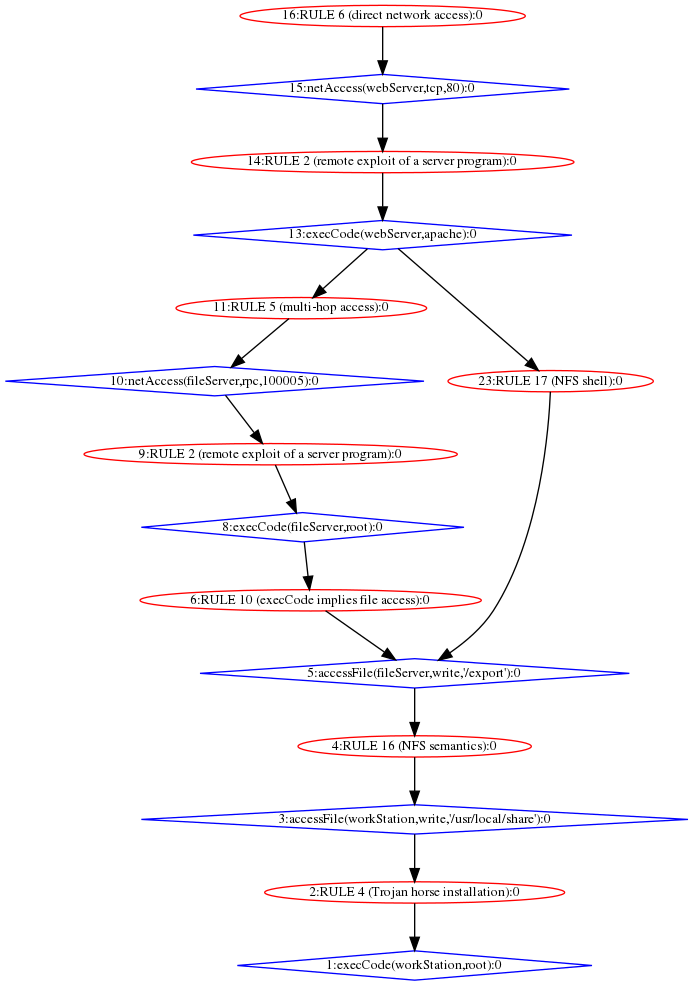
\includegraphics[width=\linewidth]{resource/img/ch_background/sdn_analytics/tmatrix_graphs/nameMe_002_pruneLEAFs.png} 
        \caption{LEAFs scored \& pruned} 
        \label{fig:tg_002}
    \end{subfigure}
          \begin{subfigure}[t]{0.3\textwidth}
        \centering
        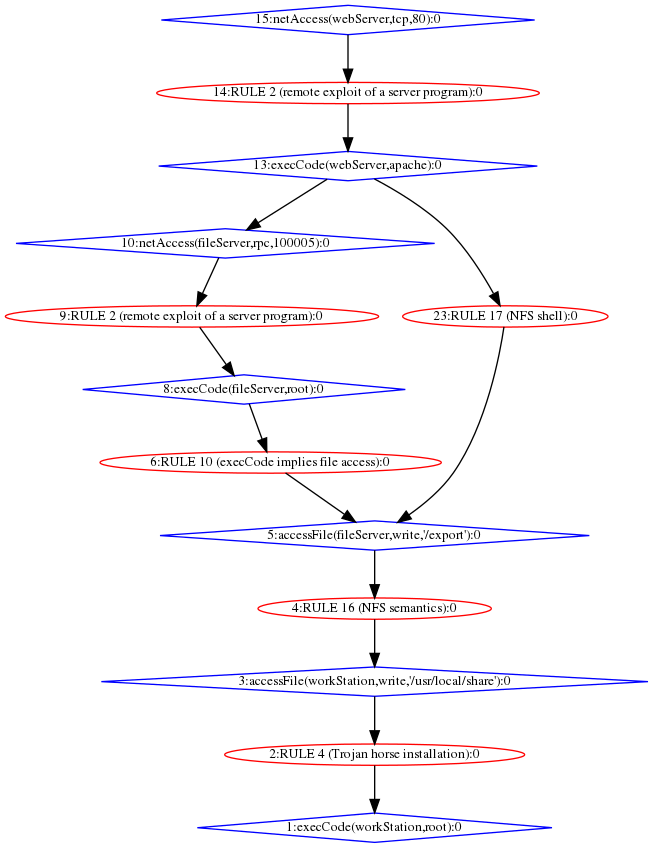
\includegraphics[width=\linewidth]{resource/img/ch_background/sdn_analytics/tmatrix_graphs/nameMe_003_coalesceANDs.png} 
        \caption{Merge non-exploit ANDs}
        \label{fig:tg_003}
    \end{subfigure}
     \begin{subfigure}[t]{0.3\textwidth}
        \centering
        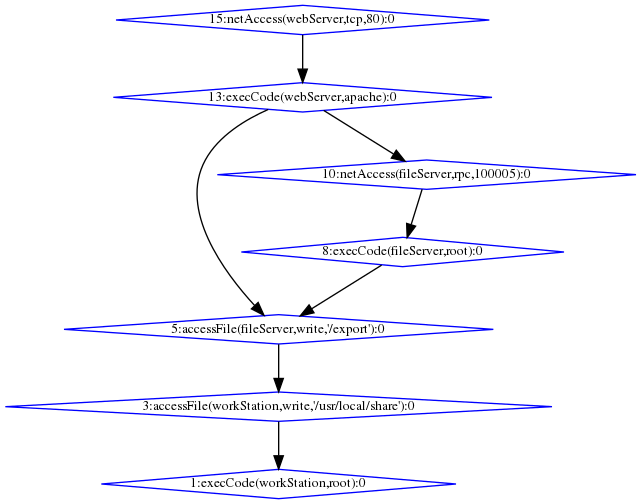
\includegraphics[width=\linewidth]{resource/img/ch_background/sdn_analytics/tmatrix_graphs/nameMe_004_scoreANDs.png} 
        \caption{Merge remaining ANDs} 
        \label{fig:tg_004}
    \end{subfigure}
    \hfill
    \vspace{.2cm}
    \centering
    \begin{subfigure}[t]{0.3\textwidth}
        \centering
        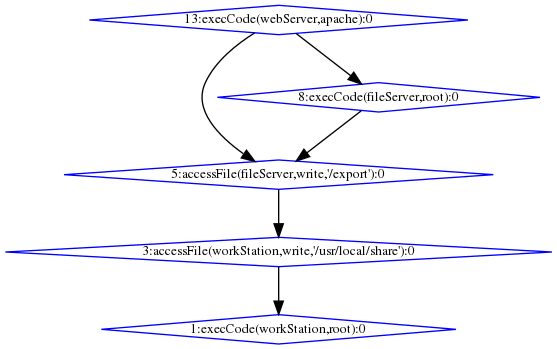
\includegraphics[width=\linewidth]{resource/img/ch_background/sdn_analytics/tmatrix_graphs/nameMe_005_coalesceORs.png} 
        \caption{Merge remaining ORs} 
        \label{fig:tg_005}
    \end{subfigure}
    \begin{subfigure}[t]{0.3\textwidth}
        \centering
        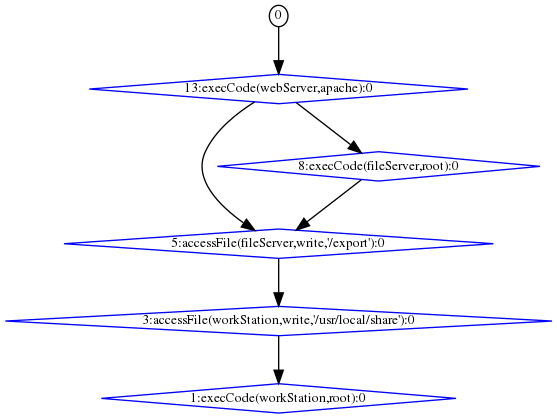
\includegraphics[width=\linewidth]{resource/img/ch_background/sdn_analytics/tmatrix_graphs/nameMe_006_addOrigin.png} 
        \caption{Add pseudo-root} 
        \label{fig:tg_006}
    \end{subfigure}
        \begin{subfigure}[t]{0.3\textwidth}
        \centering
        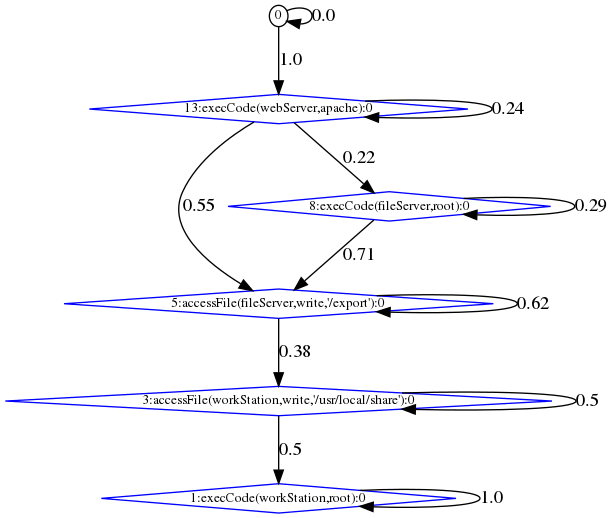
\includegraphics[width=\linewidth]{resource/img/ch_background/sdn_analytics/tmatrix_graphs/nameMe_007_weighEdges.png} 
        \caption{Calculate advance probs} 
        \label{fig:tg_008}
    \end{subfigure}
    \hfill
    \caption{Attack Graph Reduction}
    \label{fig:transGraph}
\end{figure}
